\section{Linien-Emission}
\begin{frame}{Einstein-Koeffizienten}
  \begin{columns}[T, onlytextwidth]%
    \begin{column}{0.5\textwidth}%
      \begin{tikzpicture}[
  scale=0.75,
  level/.style={very thick},
  photon/.style={-{Stealth[length=2mm]}, color=red!70!black, thick, decorate, decoration={snake, pre length=0.5mm, post length=1mm,}},
  connect/.style={dashed, very thick},
  ]
  \draw[level] (0,  0) node [left] {$E_2$} -- +(8, 0);
  \draw[level] (0, -2) node [left] {$E_1$} -- +(8, 0);
  \draw[photon] (2, 0) -- +(0,-2) node [below] {\normalcolor Emission} node[midway,left] {$A_{21}$};
  \draw[photon] (4,-2) -- +(0, 2) node [above] {\normalcolor Absortion} node[midway,left] {$B_{12}\bar{U}$};
  \draw[photon] (6, 0) -- +(0,-2) node [below] {\normalcolor stim.\ Emission} node[midway, right] {$B_{21}\bar{U}$};
  \draw[photon] (5,-1) -- +(0.95, 0);
\end{tikzpicture}
%
      Mittlere Intensität
      \vfill
      \begin{equation*}
        \bar{I} = \int_0^\infty I_ν φ(ν) \, \mathup{d}ν
      \end{equation*}
    \end{column}%
    \begin{column}{0.45\textwidth}%
      mittlere Energiedichte:
      \begin{equation*}
        \bar{U} = \frac{4\PI}{c} \bar{I},\quad\text{$\bar{I} =$ mittlere Intensität}
      \end{equation*}
      in statischem System:
      \begin{equation*}
        N_2 A_{21} + N_2 B_{21} \bar{U} = N_1 B_{12} \bar{U}
      \end{equation*}
      Mit $N_i =$ Anzahl Elektronen auf Energieniveau $E_i$
    \end{column}%
  \end{columns}%
\end{frame}

\begin{frame}{Verküpfung zu makroskopischen Größen}
  \begin{columns}[c, onlytextwidth]
    \begin{column}{0.47\textwidth}
      \textcolor{darkred}{Absorbtionskoeffizient} $\kappa_ν$ \hfill
      \begin{equation*}
        \kappa_ν = \frac{h ν}{4 \PI} N_1 B_{12} \left( 1 - \frac{g_1 N_2}{g_2 N_1} \right) φ(ν)
      \end{equation*}
    \end{column}
    \begin{column}{0.47\textwidth}
      \textcolor{darkred}{Emissionskoeffizient} $ε_ν$
      \begin{equation*}
        ε_ν = \frac{h ν}{4 \PI} N_2 A_{21} φ(ν)
      \end{equation*}
    \end{column}
  \end{columns}
  \begin{center}
    Für Radiolinien gleicht die stimulierte Emission die Absorption etwa aus. 
  \end{center}
\end{frame}

  \begin{frame}{Brightness Temperature $T_\mathup{B}$}
  \begin{align*}%
    \TB &= \frac{c²}{2 \kb} \frac{1}{ν²} I_ν & 
    \TB &= \frac{h ν}{k_\mathup{B}}
            \frac{1}{\ln\!\left(
              \frac{8\PI h ν³}{c³\bar{U}} + 1
            \right)} \\
    &\text{(allgemein)} &  &\text{(Linienemission)}
  \end{align*}%
  \begin{itemize}
    \item Rayleigh–Jeans-Temperatur für gegebene Intensität $I_ν$
    \item verbreitetes Helligkeitsmaß in der Radioastronomie
  \end{itemize}
\end{frame}

\begin{frame}[c]{Wasserstoff-Linien}%
  \begin{tikzpicture}[remember picture, overlay, shift=(current page.north)]
    \node[anchor=north] at (0, -0.9) {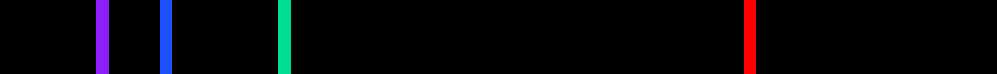
\includegraphics[width=\paperwidth]{images/H-emission-spectrum.pdf}};
  \end{tikzpicture}

  Elektrische Linienübergänge im Wasserstoff:
  \begin{equation*}
    \increment E = \frac{m e^4}{8 ε_0^2 h^2}
                    \left( \frac{1}{n_2^2} - \frac{1}{n_1^2} \right)
  \end{equation*}

  \begin{center}
  \textcolor{darkred}{Aber:} Keine starken Radiolinien.
  \end{center}
\end{frame}

\begin{frame}{Warum überhaupt Radioastronomie}
  \begin{itemize}
    \item Mittlere freie Weglänge für optisches Photon $\mathcal{O}(\si{\kilo pc})$
    \item Gasnebel und Interstellares auf großen Distanzen undurchsichtig für optisches Licht
    \item durchsichtig für Radio- und Infrarot
    \item[$\color{darkred}\Rightarrow$] einzige Möglichkeit die Struktur der Milchstraße zu vermessen
  \end{itemize}
  \begin{center}
    Deshalb: Suche nach einer Radiolinie des Wasserstoffs
  \end{center}
\end{frame}
